% Created by tikzDevice version 0.12.3.1 on 2022-02-13 15:15:12
% !TEX encoding = UTF-8 Unicode
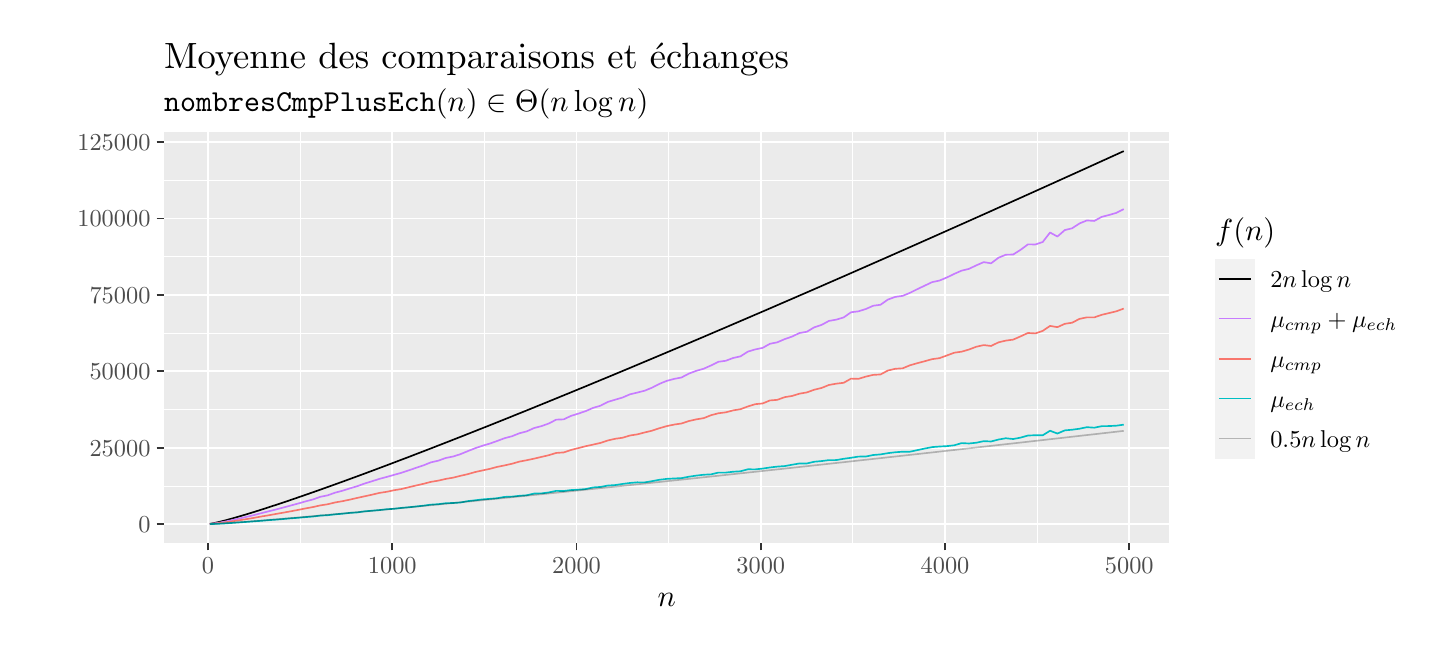
\begin{tikzpicture}[x=1pt,y=1pt]
\definecolor{fillColor}{RGB}{255,255,255}
\path[use as bounding box,fill=fillColor,fill opacity=0.00] (0,0) rectangle (505.89,216.81);
\begin{scope}
\path[clip] (  0.00,  0.00) rectangle (505.89,216.81);
\definecolor{drawColor}{RGB}{255,255,255}
\definecolor{fillColor}{RGB}{255,255,255}

\path[draw=drawColor,line width= 0.6pt,line join=round,line cap=round,fill=fillColor] (  0.00,  0.00) rectangle (505.89,216.81);
\end{scope}
\begin{scope}
\path[clip] ( 49.31, 30.69) rectangle (412.57,178.94);
\definecolor{fillColor}{gray}{0.92}

\path[fill=fillColor] ( 49.31, 30.69) rectangle (412.57,178.94);
\definecolor{drawColor}{RGB}{255,255,255}

\path[draw=drawColor,line width= 0.3pt,line join=round] ( 49.31, 51.22) --
	(412.57, 51.22);

\path[draw=drawColor,line width= 0.3pt,line join=round] ( 49.31, 78.83) --
	(412.57, 78.83);

\path[draw=drawColor,line width= 0.3pt,line join=round] ( 49.31,106.43) --
	(412.57,106.43);

\path[draw=drawColor,line width= 0.3pt,line join=round] ( 49.31,134.04) --
	(412.57,134.04);

\path[draw=drawColor,line width= 0.3pt,line join=round] ( 49.31,161.65) --
	(412.57,161.65);

\path[draw=drawColor,line width= 0.3pt,line join=round] ( 98.44, 30.69) --
	( 98.44,178.94);

\path[draw=drawColor,line width= 0.3pt,line join=round] (165.03, 30.69) --
	(165.03,178.94);

\path[draw=drawColor,line width= 0.3pt,line join=round] (231.61, 30.69) --
	(231.61,178.94);

\path[draw=drawColor,line width= 0.3pt,line join=round] (298.19, 30.69) --
	(298.19,178.94);

\path[draw=drawColor,line width= 0.3pt,line join=round] (364.77, 30.69) --
	(364.77,178.94);

\path[draw=drawColor,line width= 0.6pt,line join=round] ( 49.31, 37.41) --
	(412.57, 37.41);

\path[draw=drawColor,line width= 0.6pt,line join=round] ( 49.31, 65.02) --
	(412.57, 65.02);

\path[draw=drawColor,line width= 0.6pt,line join=round] ( 49.31, 92.63) --
	(412.57, 92.63);

\path[draw=drawColor,line width= 0.6pt,line join=round] ( 49.31,120.24) --
	(412.57,120.24);

\path[draw=drawColor,line width= 0.6pt,line join=round] ( 49.31,147.85) --
	(412.57,147.85);

\path[draw=drawColor,line width= 0.6pt,line join=round] ( 49.31,175.45) --
	(412.57,175.45);

\path[draw=drawColor,line width= 0.6pt,line join=round] ( 65.15, 30.69) --
	( 65.15,178.94);

\path[draw=drawColor,line width= 0.6pt,line join=round] (131.74, 30.69) --
	(131.74,178.94);

\path[draw=drawColor,line width= 0.6pt,line join=round] (198.32, 30.69) --
	(198.32,178.94);

\path[draw=drawColor,line width= 0.6pt,line join=round] (264.90, 30.69) --
	(264.90,178.94);

\path[draw=drawColor,line width= 0.6pt,line join=round] (331.48, 30.69) --
	(331.48,178.94);

\path[draw=drawColor,line width= 0.6pt,line join=round] (398.06, 30.69) --
	(398.06,178.94);
\definecolor{drawColor}{RGB}{0,0,0}

\path[draw=drawColor,line width= 0.6pt,line join=round] ( 65.82, 37.49) --
	( 68.48, 38.04) --
	( 71.15, 38.70) --
	( 73.81, 39.43) --
	( 76.47, 40.20) --
	( 79.14, 40.99) --
	( 81.80, 41.81) --
	( 84.46, 42.65) --
	( 87.13, 43.51) --
	( 89.79, 44.39) --
	( 92.45, 45.27) --
	( 95.12, 46.17) --
	( 97.78, 47.09) --
	(100.44, 48.01) --
	(103.11, 48.94) --
	(105.77, 49.88) --
	(108.43, 50.83) --
	(111.10, 51.79) --
	(113.76, 52.75) --
	(116.42, 53.72) --
	(119.09, 54.70) --
	(121.75, 55.68) --
	(124.41, 56.67) --
	(127.07, 57.67) --
	(129.74, 58.67) --
	(132.40, 59.68) --
	(135.06, 60.69) --
	(137.73, 61.70) --
	(140.39, 62.73) --
	(143.05, 63.75) --
	(145.72, 64.78) --
	(148.38, 65.82) --
	(151.04, 66.85) --
	(153.71, 67.90) --
	(156.37, 68.94) --
	(159.03, 69.99) --
	(161.70, 71.05) --
	(164.36, 72.10) --
	(167.02, 73.16) --
	(169.69, 74.23) --
	(172.35, 75.29) --
	(175.01, 76.36) --
	(177.68, 77.44) --
	(180.34, 78.51) --
	(183.00, 79.59) --
	(185.67, 80.68) --
	(188.33, 81.76) --
	(190.99, 82.85) --
	(193.66, 83.94) --
	(196.32, 85.03) --
	(198.98, 86.13) --
	(201.65, 87.22) --
	(204.31, 88.33) --
	(206.97, 89.43) --
	(209.64, 90.53) --
	(212.30, 91.64) --
	(214.96, 92.75) --
	(217.63, 93.86) --
	(220.29, 94.98) --
	(222.95, 96.10) --
	(225.61, 97.21) --
	(228.28, 98.34) --
	(230.94, 99.46) --
	(233.60,100.58) --
	(236.27,101.71) --
	(238.93,102.84) --
	(241.59,103.97) --
	(244.26,105.10) --
	(246.92,106.24) --
	(249.58,107.38) --
	(252.25,108.51) --
	(254.91,109.66) --
	(257.57,110.80) --
	(260.24,111.94) --
	(262.90,113.09) --
	(265.56,114.23) --
	(268.23,115.38) --
	(270.89,116.54) --
	(273.55,117.69) --
	(276.22,118.84) --
	(278.88,120.00) --
	(281.54,121.15) --
	(284.21,122.31) --
	(286.87,123.47) --
	(289.53,124.64) --
	(292.20,125.80) --
	(294.86,126.96) --
	(297.52,128.13) --
	(300.19,129.30) --
	(302.85,130.47) --
	(305.51,131.64) --
	(308.18,132.81) --
	(310.84,133.98) --
	(313.50,135.16) --
	(316.17,136.34) --
	(318.83,137.51) --
	(321.49,138.69) --
	(324.15,139.87) --
	(326.82,141.05) --
	(329.48,142.24) --
	(332.14,143.42) --
	(334.81,144.61) --
	(337.47,145.79) --
	(340.13,146.98) --
	(342.80,148.17) --
	(345.46,149.36) --
	(348.12,150.55) --
	(350.79,151.75) --
	(353.45,152.94) --
	(356.11,154.14) --
	(358.78,155.33) --
	(361.44,156.53) --
	(364.10,157.73) --
	(366.77,158.93) --
	(369.43,160.13) --
	(372.09,161.33) --
	(374.76,162.54) --
	(377.42,163.74) --
	(380.08,164.94) --
	(382.75,166.15) --
	(385.41,167.36) --
	(388.07,168.57) --
	(390.74,169.78) --
	(393.40,170.99) --
	(396.06,172.20);
\definecolor{drawColor}{RGB}{199,124,255}

\path[draw=drawColor,line width= 0.6pt,line join=round] ( 65.82, 37.45) --
	( 68.48, 37.81) --
	( 71.15, 38.29) --
	( 73.81, 38.85) --
	( 76.47, 39.44) --
	( 79.14, 40.05) --
	( 81.80, 40.70) --
	( 84.46, 41.39) --
	( 87.13, 42.06) --
	( 89.79, 42.73) --
	( 92.45, 43.43) --
	( 95.12, 44.16) --
	( 97.78, 44.87) --
	(100.44, 45.64) --
	(103.11, 46.34) --
	(105.77, 47.29) --
	(108.43, 47.83) --
	(111.10, 48.79) --
	(113.76, 49.48) --
	(116.42, 50.33) --
	(119.09, 51.12) --
	(121.75, 52.09) --
	(124.41, 52.90) --
	(127.07, 53.76) --
	(129.74, 54.47) --
	(132.40, 55.22) --
	(135.06, 55.97) --
	(137.73, 56.85) --
	(140.39, 57.78) --
	(143.05, 58.66) --
	(145.72, 59.74) --
	(148.38, 60.34) --
	(151.04, 61.31) --
	(153.71, 61.84) --
	(156.37, 62.69) --
	(159.03, 63.79) --
	(161.70, 64.85) --
	(164.36, 65.75) --
	(167.02, 66.53) --
	(169.69, 67.48) --
	(172.35, 68.48) --
	(175.01, 69.17) --
	(177.68, 70.25) --
	(180.34, 70.93) --
	(183.00, 72.14) --
	(185.67, 72.83) --
	(188.33, 73.79) --
	(190.99, 75.17) --
	(193.66, 75.27) --
	(196.32, 76.52) --
	(198.98, 77.35) --
	(201.65, 78.26) --
	(204.31, 79.42) --
	(206.97, 80.20) --
	(209.64, 81.58) --
	(212.30, 82.38) --
	(214.96, 83.16) --
	(217.63, 84.32) --
	(220.29, 84.95) --
	(222.95, 85.63) --
	(225.61, 86.72) --
	(228.28, 88.10) --
	(230.94, 89.19) --
	(233.60, 89.89) --
	(236.27, 90.41) --
	(238.93, 91.81) --
	(241.59, 92.81) --
	(244.26, 93.56) --
	(246.92, 94.75) --
	(249.58, 96.08) --
	(252.25, 96.44) --
	(254.91, 97.45) --
	(257.57, 98.04) --
	(260.24, 99.75) --
	(262.90,100.55) --
	(265.56,101.09) --
	(268.23,102.59) --
	(270.89,103.12) --
	(273.55,104.27) --
	(276.22,105.19) --
	(278.88,106.47) --
	(281.54,106.93) --
	(284.21,108.53) --
	(286.87,109.41) --
	(289.53,110.84) --
	(292.20,111.31) --
	(294.86,112.11) --
	(297.52,113.97) --
	(300.19,114.31) --
	(302.85,115.14) --
	(305.51,116.32) --
	(308.18,116.69) --
	(310.84,118.56) --
	(313.50,119.53) --
	(316.17,119.89) --
	(318.83,121.00) --
	(321.49,122.33) --
	(324.15,123.59) --
	(326.82,124.86) --
	(329.48,125.43) --
	(332.14,126.54) --
	(334.81,127.84) --
	(337.47,129.01) --
	(340.13,129.65) --
	(342.80,130.93) --
	(345.46,132.09) --
	(348.12,131.66) --
	(350.79,133.67) --
	(353.45,134.77) --
	(356.11,134.84) --
	(358.78,136.53) --
	(361.44,138.51) --
	(364.10,138.47) --
	(366.77,139.34) --
	(369.43,142.79) --
	(372.09,141.33) --
	(374.76,143.67) --
	(377.42,144.32) --
	(380.08,146.07) --
	(382.75,147.16) --
	(385.41,146.97) --
	(388.07,148.43) --
	(390.74,149.12) --
	(393.40,149.89) --
	(396.06,151.26);
\definecolor{drawColor}{RGB}{248,118,109}

\path[draw=drawColor,line width= 0.6pt,line join=round] ( 65.82, 37.44) --
	( 68.48, 37.70) --
	( 71.15, 38.03) --
	( 73.81, 38.41) --
	( 76.47, 38.82) --
	( 79.14, 39.24) --
	( 81.80, 39.69) --
	( 84.46, 40.18) --
	( 87.13, 40.62) --
	( 89.79, 41.11) --
	( 92.45, 41.57) --
	( 95.12, 42.06) --
	( 97.78, 42.57) --
	(100.44, 43.10) --
	(103.11, 43.59) --
	(105.77, 44.19) --
	(108.43, 44.60) --
	(111.10, 45.25) --
	(113.76, 45.71) --
	(116.42, 46.27) --
	(119.09, 46.89) --
	(121.75, 47.47) --
	(124.41, 48.05) --
	(127.07, 48.69) --
	(129.74, 49.10) --
	(132.40, 49.67) --
	(135.06, 50.10) --
	(137.73, 50.75) --
	(140.39, 51.39) --
	(143.05, 51.99) --
	(145.72, 52.69) --
	(148.38, 53.13) --
	(151.04, 53.75) --
	(153.71, 54.20) --
	(156.37, 54.87) --
	(159.03, 55.47) --
	(161.70, 56.24) --
	(164.36, 56.82) --
	(167.02, 57.39) --
	(169.69, 58.11) --
	(172.35, 58.64) --
	(175.01, 59.23) --
	(177.68, 60.01) --
	(180.34, 60.51) --
	(183.00, 61.08) --
	(185.67, 61.71) --
	(188.33, 62.33) --
	(190.99, 63.14) --
	(193.66, 63.32) --
	(196.32, 64.21) --
	(198.98, 64.89) --
	(201.65, 65.58) --
	(204.31, 66.15) --
	(206.97, 66.76) --
	(209.64, 67.64) --
	(212.30, 68.26) --
	(214.96, 68.63) --
	(217.63, 69.44) --
	(220.29, 69.85) --
	(222.95, 70.54) --
	(225.61, 71.18) --
	(228.28, 72.07) --
	(230.94, 72.84) --
	(233.60, 73.39) --
	(236.27, 73.78) --
	(238.93, 74.67) --
	(241.59, 75.27) --
	(244.26, 75.71) --
	(246.92, 76.77) --
	(249.58, 77.47) --
	(252.25, 77.81) --
	(254.91, 78.51) --
	(257.57, 78.95) --
	(260.24, 79.94) --
	(262.90, 80.76) --
	(265.56, 81.02) --
	(268.23, 82.11) --
	(270.89, 82.33) --
	(273.55, 83.30) --
	(276.22, 83.73) --
	(278.88, 84.55) --
	(281.54, 85.01) --
	(284.21, 85.98) --
	(286.87, 86.62) --
	(289.53, 87.70) --
	(292.20, 88.17) --
	(294.86, 88.49) --
	(297.52, 89.99) --
	(300.19, 89.91) --
	(302.85, 90.72) --
	(305.51, 91.34) --
	(308.18, 91.50) --
	(310.84, 92.92) --
	(313.50, 93.55) --
	(316.17, 93.72) --
	(318.83, 94.82) --
	(321.49, 95.58) --
	(324.15, 96.28) --
	(326.82, 97.03) --
	(329.48, 97.39) --
	(332.14, 98.36) --
	(334.81, 99.35) --
	(337.47, 99.73) --
	(340.13,100.51) --
	(342.80,101.52) --
	(345.46,102.11) --
	(348.12,101.79) --
	(350.79,103.10) --
	(353.45,103.73) --
	(356.11,104.09) --
	(358.78,105.26) --
	(361.44,106.49) --
	(364.10,106.34) --
	(366.77,107.24) --
	(369.43,109.04) --
	(372.09,108.59) --
	(374.76,109.80) --
	(377.42,110.20) --
	(380.08,111.59) --
	(382.75,112.13) --
	(385.41,112.12) --
	(388.07,113.04) --
	(390.74,113.68) --
	(393.40,114.32) --
	(396.06,115.31);
\definecolor{drawColor}{RGB}{0,191,196}

\path[draw=drawColor,line width= 0.6pt,line join=round] ( 65.82, 37.42) --
	( 68.48, 37.53) --
	( 71.15, 37.67) --
	( 73.81, 37.85) --
	( 76.47, 38.04) --
	( 79.14, 38.22) --
	( 81.80, 38.43) --
	( 84.46, 38.62) --
	( 87.13, 38.86) --
	( 89.79, 39.04) --
	( 92.45, 39.27) --
	( 95.12, 39.52) --
	( 97.78, 39.71) --
	(100.44, 39.96) --
	(103.11, 40.16) --
	(105.77, 40.51) --
	(108.43, 40.64) --
	(111.10, 40.95) --
	(113.76, 41.18) --
	(116.42, 41.48) --
	(119.09, 41.64) --
	(121.75, 42.04) --
	(124.41, 42.26) --
	(127.07, 42.49) --
	(129.74, 42.79) --
	(132.40, 42.96) --
	(135.06, 43.28) --
	(137.73, 43.51) --
	(140.39, 43.80) --
	(143.05, 44.09) --
	(145.72, 44.46) --
	(148.38, 44.62) --
	(151.04, 44.97) --
	(153.71, 45.05) --
	(156.37, 45.23) --
	(159.03, 45.73) --
	(161.70, 46.03) --
	(164.36, 46.35) --
	(167.02, 46.55) --
	(169.69, 46.78) --
	(172.35, 47.26) --
	(175.01, 47.35) --
	(177.68, 47.65) --
	(180.34, 47.84) --
	(183.00, 48.47) --
	(185.67, 48.53) --
	(188.33, 48.87) --
	(190.99, 49.44) --
	(193.66, 49.37) --
	(196.32, 49.72) --
	(198.98, 49.87) --
	(201.65, 50.09) --
	(204.31, 50.68) --
	(206.97, 50.85) --
	(209.64, 51.36) --
	(212.30, 51.53) --
	(214.96, 51.94) --
	(217.63, 52.29) --
	(220.29, 52.52) --
	(222.95, 52.50) --
	(225.61, 52.95) --
	(228.28, 53.44) --
	(230.94, 53.77) --
	(233.60, 53.91) --
	(236.27, 54.05) --
	(238.93, 54.55) --
	(241.59, 54.95) --
	(244.26, 55.26) --
	(246.92, 55.40) --
	(249.58, 56.03) --
	(252.25, 56.04) --
	(254.91, 56.35) --
	(257.57, 56.51) --
	(260.24, 57.23) --
	(262.90, 57.20) --
	(265.56, 57.48) --
	(268.23, 57.89) --
	(270.89, 58.20) --
	(273.55, 58.39) --
	(276.22, 58.88) --
	(278.88, 59.34) --
	(281.54, 59.33) --
	(284.21, 59.96) --
	(286.87, 60.20) --
	(289.53, 60.55) --
	(292.20, 60.56) --
	(294.86, 61.03) --
	(297.52, 61.39) --
	(300.19, 61.82) --
	(302.85, 61.84) --
	(305.51, 62.39) --
	(308.18, 62.61) --
	(310.84, 63.06) --
	(313.50, 63.39) --
	(316.17, 63.58) --
	(318.83, 63.59) --
	(321.49, 64.16) --
	(324.15, 64.73) --
	(326.82, 65.25) --
	(329.48, 65.46) --
	(332.14, 65.60) --
	(334.81, 65.90) --
	(337.47, 66.69) --
	(340.13, 66.56) --
	(342.80, 66.83) --
	(345.46, 67.40) --
	(348.12, 67.28) --
	(350.79, 67.98) --
	(353.45, 68.45) --
	(356.11, 68.16) --
	(358.78, 68.68) --
	(361.44, 69.43) --
	(364.10, 69.54) --
	(366.77, 69.51) --
	(369.43, 71.16) --
	(372.09, 70.15) --
	(374.76, 71.29) --
	(377.42, 71.53) --
	(380.08, 71.89) --
	(382.75, 72.45) --
	(385.41, 72.26) --
	(388.07, 72.81) --
	(390.74, 72.85) --
	(393.40, 72.99) --
	(396.06, 73.36);
\definecolor{drawColor}{RGB}{0,0,0}

\path[draw=drawColor,draw opacity=0.25,line width= 0.6pt,line join=round] ( 65.82, 37.43) --
	( 68.48, 37.57) --
	( 71.15, 37.74) --
	( 73.81, 37.92) --
	( 76.47, 38.11) --
	( 79.14, 38.31) --
	( 81.80, 38.51) --
	( 84.46, 38.72) --
	( 87.13, 38.94) --
	( 89.79, 39.16) --
	( 92.45, 39.38) --
	( 95.12, 39.60) --
	( 97.78, 39.83) --
	(100.44, 40.06) --
	(103.11, 40.30) --
	(105.77, 40.53) --
	(108.43, 40.77) --
	(111.10, 41.01) --
	(113.76, 41.25) --
	(116.42, 41.49) --
	(119.09, 41.74) --
	(121.75, 41.98) --
	(124.41, 42.23) --
	(127.07, 42.48) --
	(129.74, 42.73) --
	(132.40, 42.98) --
	(135.06, 43.23) --
	(137.73, 43.49) --
	(140.39, 43.74) --
	(143.05, 44.00) --
	(145.72, 44.26) --
	(148.38, 44.51) --
	(151.04, 44.77) --
	(153.71, 45.03) --
	(156.37, 45.30) --
	(159.03, 45.56) --
	(161.70, 45.82) --
	(164.36, 46.09) --
	(167.02, 46.35) --
	(169.69, 46.62) --
	(172.35, 46.88) --
	(175.01, 47.15) --
	(177.68, 47.42) --
	(180.34, 47.69) --
	(183.00, 47.96) --
	(185.67, 48.23) --
	(188.33, 48.50) --
	(190.99, 48.77) --
	(193.66, 49.04) --
	(196.32, 49.32) --
	(198.98, 49.59) --
	(201.65, 49.87) --
	(204.31, 50.14) --
	(206.97, 50.42) --
	(209.64, 50.69) --
	(212.30, 50.97) --
	(214.96, 51.25) --
	(217.63, 51.53) --
	(220.29, 51.81) --
	(222.95, 52.08) --
	(225.61, 52.36) --
	(228.28, 52.64) --
	(230.94, 52.93) --
	(233.60, 53.21) --
	(236.27, 53.49) --
	(238.93, 53.77) --
	(241.59, 54.05) --
	(244.26, 54.34) --
	(246.92, 54.62) --
	(249.58, 54.90) --
	(252.25, 55.19) --
	(254.91, 55.47) --
	(257.57, 55.76) --
	(260.24, 56.05) --
	(262.90, 56.33) --
	(265.56, 56.62) --
	(268.23, 56.91) --
	(270.89, 57.19) --
	(273.55, 57.48) --
	(276.22, 57.77) --
	(278.88, 58.06) --
	(281.54, 58.35) --
	(284.21, 58.64) --
	(286.87, 58.93) --
	(289.53, 59.22) --
	(292.20, 59.51) --
	(294.86, 59.80) --
	(297.52, 60.09) --
	(300.19, 60.39) --
	(302.85, 60.68) --
	(305.51, 60.97) --
	(308.18, 61.26) --
	(310.84, 61.56) --
	(313.50, 61.85) --
	(316.17, 62.14) --
	(318.83, 62.44) --
	(321.49, 62.73) --
	(324.15, 63.03) --
	(326.82, 63.32) --
	(329.48, 63.62) --
	(332.14, 63.92) --
	(334.81, 64.21) --
	(337.47, 64.51) --
	(340.13, 64.81) --
	(342.80, 65.10) --
	(345.46, 65.40) --
	(348.12, 65.70) --
	(350.79, 66.00) --
	(353.45, 66.30) --
	(356.11, 66.59) --
	(358.78, 66.89) --
	(361.44, 67.19) --
	(364.10, 67.49) --
	(366.77, 67.79) --
	(369.43, 68.09) --
	(372.09, 68.39) --
	(374.76, 68.69) --
	(377.42, 69.00) --
	(380.08, 69.30) --
	(382.75, 69.60) --
	(385.41, 69.90) --
	(388.07, 70.20) --
	(390.74, 70.50) --
	(393.40, 70.81) --
	(396.06, 71.11);
\end{scope}
\begin{scope}
\path[clip] (  0.00,  0.00) rectangle (505.89,216.81);
\definecolor{drawColor}{gray}{0.30}

\node[text=drawColor,anchor=base east,inner sep=0pt, outer sep=0pt, scale=  0.88] at ( 44.36, 34.38) {0};

\node[text=drawColor,anchor=base east,inner sep=0pt, outer sep=0pt, scale=  0.88] at ( 44.36, 61.99) {25000};

\node[text=drawColor,anchor=base east,inner sep=0pt, outer sep=0pt, scale=  0.88] at ( 44.36, 89.60) {50000};

\node[text=drawColor,anchor=base east,inner sep=0pt, outer sep=0pt, scale=  0.88] at ( 44.36,117.21) {75000};

\node[text=drawColor,anchor=base east,inner sep=0pt, outer sep=0pt, scale=  0.88] at ( 44.36,144.82) {100000};

\node[text=drawColor,anchor=base east,inner sep=0pt, outer sep=0pt, scale=  0.88] at ( 44.36,172.42) {125000};
\end{scope}
\begin{scope}
\path[clip] (  0.00,  0.00) rectangle (505.89,216.81);
\definecolor{drawColor}{gray}{0.20}

\path[draw=drawColor,line width= 0.6pt,line join=round] ( 46.56, 37.41) --
	( 49.31, 37.41);

\path[draw=drawColor,line width= 0.6pt,line join=round] ( 46.56, 65.02) --
	( 49.31, 65.02);

\path[draw=drawColor,line width= 0.6pt,line join=round] ( 46.56, 92.63) --
	( 49.31, 92.63);

\path[draw=drawColor,line width= 0.6pt,line join=round] ( 46.56,120.24) --
	( 49.31,120.24);

\path[draw=drawColor,line width= 0.6pt,line join=round] ( 46.56,147.85) --
	( 49.31,147.85);

\path[draw=drawColor,line width= 0.6pt,line join=round] ( 46.56,175.45) --
	( 49.31,175.45);
\end{scope}
\begin{scope}
\path[clip] (  0.00,  0.00) rectangle (505.89,216.81);
\definecolor{drawColor}{gray}{0.20}

\path[draw=drawColor,line width= 0.6pt,line join=round] ( 65.15, 27.94) --
	( 65.15, 30.69);

\path[draw=drawColor,line width= 0.6pt,line join=round] (131.74, 27.94) --
	(131.74, 30.69);

\path[draw=drawColor,line width= 0.6pt,line join=round] (198.32, 27.94) --
	(198.32, 30.69);

\path[draw=drawColor,line width= 0.6pt,line join=round] (264.90, 27.94) --
	(264.90, 30.69);

\path[draw=drawColor,line width= 0.6pt,line join=round] (331.48, 27.94) --
	(331.48, 30.69);

\path[draw=drawColor,line width= 0.6pt,line join=round] (398.06, 27.94) --
	(398.06, 30.69);
\end{scope}
\begin{scope}
\path[clip] (  0.00,  0.00) rectangle (505.89,216.81);
\definecolor{drawColor}{gray}{0.30}

\node[text=drawColor,anchor=base,inner sep=0pt, outer sep=0pt, scale=  0.88] at ( 65.15, 19.68) {0};

\node[text=drawColor,anchor=base,inner sep=0pt, outer sep=0pt, scale=  0.88] at (131.74, 19.68) {1000};

\node[text=drawColor,anchor=base,inner sep=0pt, outer sep=0pt, scale=  0.88] at (198.32, 19.68) {2000};

\node[text=drawColor,anchor=base,inner sep=0pt, outer sep=0pt, scale=  0.88] at (264.90, 19.68) {3000};

\node[text=drawColor,anchor=base,inner sep=0pt, outer sep=0pt, scale=  0.88] at (331.48, 19.68) {4000};

\node[text=drawColor,anchor=base,inner sep=0pt, outer sep=0pt, scale=  0.88] at (398.06, 19.68) {5000};
\end{scope}
\begin{scope}
\path[clip] (  0.00,  0.00) rectangle (505.89,216.81);
\definecolor{drawColor}{RGB}{0,0,0}

\node[text=drawColor,anchor=base,inner sep=0pt, outer sep=0pt, scale=  1.10] at (230.94,  7.64) {$n$};
\end{scope}
\begin{scope}
\path[clip] (  0.00,  0.00) rectangle (505.89,216.81);
\definecolor{fillColor}{RGB}{255,255,255}

\path[fill=fillColor] (423.57, 55.57) rectangle (500.39,154.05);
\end{scope}
\begin{scope}
\path[clip] (  0.00,  0.00) rectangle (505.89,216.81);
\definecolor{drawColor}{RGB}{0,0,0}

\node[text=drawColor,anchor=base west,inner sep=0pt, outer sep=0pt, scale=  1.10] at (429.07,139.91) {$f(n)$};
\end{scope}
\begin{scope}
\path[clip] (  0.00,  0.00) rectangle (505.89,216.81);
\definecolor{fillColor}{gray}{0.95}

\path[fill=fillColor] (429.07,118.89) rectangle (443.53,133.34);
\end{scope}
\begin{scope}
\path[clip] (  0.00,  0.00) rectangle (505.89,216.81);
\definecolor{drawColor}{RGB}{0,0,0}

\path[draw=drawColor,line width= 0.6pt,line join=round] (430.52,126.11) -- (442.08,126.11);
\end{scope}
\begin{scope}
\path[clip] (  0.00,  0.00) rectangle (505.89,216.81);
\definecolor{fillColor}{gray}{0.95}

\path[fill=fillColor] (429.07,104.43) rectangle (443.53,118.89);
\end{scope}
\begin{scope}
\path[clip] (  0.00,  0.00) rectangle (505.89,216.81);
\definecolor{drawColor}{RGB}{199,124,255}

\path[draw=drawColor,line width= 0.6pt,line join=round] (430.52,111.66) -- (442.08,111.66);
\end{scope}
\begin{scope}
\path[clip] (  0.00,  0.00) rectangle (505.89,216.81);
\definecolor{fillColor}{gray}{0.95}

\path[fill=fillColor] (429.07, 89.98) rectangle (443.53,104.43);
\end{scope}
\begin{scope}
\path[clip] (  0.00,  0.00) rectangle (505.89,216.81);
\definecolor{drawColor}{RGB}{248,118,109}

\path[draw=drawColor,line width= 0.6pt,line join=round] (430.52, 97.20) -- (442.08, 97.20);
\end{scope}
\begin{scope}
\path[clip] (  0.00,  0.00) rectangle (505.89,216.81);
\definecolor{fillColor}{gray}{0.95}

\path[fill=fillColor] (429.07, 75.52) rectangle (443.53, 89.98);
\end{scope}
\begin{scope}
\path[clip] (  0.00,  0.00) rectangle (505.89,216.81);
\definecolor{drawColor}{RGB}{0,191,196}

\path[draw=drawColor,line width= 0.6pt,line join=round] (430.52, 82.75) -- (442.08, 82.75);
\end{scope}
\begin{scope}
\path[clip] (  0.00,  0.00) rectangle (505.89,216.81);
\definecolor{fillColor}{gray}{0.95}

\path[fill=fillColor] (429.07, 61.07) rectangle (443.53, 75.52);
\end{scope}
\begin{scope}
\path[clip] (  0.00,  0.00) rectangle (505.89,216.81);
\definecolor{drawColor}{RGB}{0,0,0}

\path[draw=drawColor,draw opacity=0.25,line width= 0.6pt,line join=round] (430.52, 68.30) -- (442.08, 68.30);
\end{scope}
\begin{scope}
\path[clip] (  0.00,  0.00) rectangle (505.89,216.81);
\definecolor{drawColor}{RGB}{0,0,0}

\node[text=drawColor,anchor=base west,inner sep=0pt, outer sep=0pt, scale=  0.88] at (449.03,123.08) {$2n \log n$};
\end{scope}
\begin{scope}
\path[clip] (  0.00,  0.00) rectangle (505.89,216.81);
\definecolor{drawColor}{RGB}{0,0,0}

\node[text=drawColor,anchor=base west,inner sep=0pt, outer sep=0pt, scale=  0.88] at (449.03,108.63) {$\mu_{cmp} + \mu_{ech}$};
\end{scope}
\begin{scope}
\path[clip] (  0.00,  0.00) rectangle (505.89,216.81);
\definecolor{drawColor}{RGB}{0,0,0}

\node[text=drawColor,anchor=base west,inner sep=0pt, outer sep=0pt, scale=  0.88] at (449.03, 94.17) {$\mu_{cmp}$};
\end{scope}
\begin{scope}
\path[clip] (  0.00,  0.00) rectangle (505.89,216.81);
\definecolor{drawColor}{RGB}{0,0,0}

\node[text=drawColor,anchor=base west,inner sep=0pt, outer sep=0pt, scale=  0.88] at (449.03, 79.72) {$\mu_{ech}$};
\end{scope}
\begin{scope}
\path[clip] (  0.00,  0.00) rectangle (505.89,216.81);
\definecolor{drawColor}{RGB}{0,0,0}

\node[text=drawColor,anchor=base west,inner sep=0pt, outer sep=0pt, scale=  0.88] at (449.03, 65.27) {$0.5n \log n$};
\end{scope}
\begin{scope}
\path[clip] (  0.00,  0.00) rectangle (505.89,216.81);
\definecolor{drawColor}{RGB}{0,0,0}

\node[text=drawColor,anchor=base west,inner sep=0pt, outer sep=0pt, scale=  1.10] at ( 49.31,186.58) {$\texttt{nombresCmpPlusEch}(n) \in \Theta(n \log n)$};
\end{scope}
\begin{scope}
\path[clip] (  0.00,  0.00) rectangle (505.89,216.81);
\definecolor{drawColor}{RGB}{0,0,0}

\node[text=drawColor,anchor=base west,inner sep=0pt, outer sep=0pt, scale=  1.32] at ( 49.31,202.22) {Moyenne des comparaisons et échanges};
\end{scope}
\end{tikzpicture}
